\PassOptionsToPackage{unicode=true}{hyperref} % options for packages loaded elsewhere
\PassOptionsToPackage{hyphens}{url}
%
\documentclass[10pt,xcolor=table,color={dvipsnames,usenames},ignorenonframetext,usepdftitle=false,english]{beamer}
\setbeamertemplate{caption}[numbered]
\setbeamertemplate{caption label separator}{: }
\setbeamercolor{caption name}{fg=normal text.fg}
\beamertemplatenavigationsymbolsempty
\usepackage{caption}
\captionsetup{skip=0pt,belowskip=0pt}
%\setlength\abovecaptionskip{-15pt}
\usepackage{lmodern}
\usepackage{amssymb,amsmath,mathtools,multirow}
\usepackage{float,hhline}
\usepackage{tikz}
\usepackage{mathtools}
\usepackage{ifxetex,ifluatex}
\usepackage{fixltx2e} % provides \textsubscript
\ifnum 0\ifxetex 1\fi\ifluatex 1\fi=0 % if pdftex
  \usepackage[T1]{fontenc}
  \usepackage[utf8]{inputenc}
  \usepackage{textcomp} % provides euro and other symbols
\else % if luatex or xelatex
  \usepackage{unicode-math}
  \defaultfontfeatures{Ligatures=TeX,Scale=MatchLowercase}
\fi
\usetheme[coding=utf8,language=english,
,titlepagelogo=img/logojsm.png
]{TorinoTh}
% use upquote if available, for straight quotes in verbatim environments
\IfFileExists{upquote.sty}{\usepackage{upquote}}{}
% use microtype if available
\IfFileExists{microtype.sty}{%
\usepackage[]{microtype}
\UseMicrotypeSet[protrusion]{basicmath} % disable protrusion for tt fonts
}{}
\IfFileExists{parskip.sty}{%
\usepackage{parskip}
}{% else
\setlength{\parindent}{0pt}
\setlength{\parskip}{6pt plus 2pt minus 1pt}
}
\usepackage{hyperref}
\hypersetup{
            pdfauthor={Alain Quartier-la-Tente (Lemna, Insee)},
            pdfborder={0 0 0},
            breaklinks=true}
\urlstyle{same}  % don't use monospace font for urls
\newif\ifbibliography
\newlength{\cslhangindent}
\setlength{\cslhangindent}{1.5em}
\newlength{\csllabelwidth}
\setlength{\csllabelwidth}{3em}
\newenvironment{CSLReferences}[2] % #1 hanging-ident, #2 entry spacing
 {% don't indent paragraphs
  \setlength{\parindent}{0pt}
  % turn on hanging indent if param 1 is 1
  \ifodd #1 \everypar{\setlength{\hangindent}{\cslhangindent}}\ignorespaces\fi
  % set entry spacing
  \ifnum #2 > 0
  \setlength{\parskip}{#2\baselineskip}
  \fi
 }%
 {}
\usepackage{color}
\usepackage{fancyvrb}
\newcommand{\VerbBar}{|}
\newcommand{\VERB}{\Verb[commandchars=\\\{\}]}
\DefineVerbatimEnvironment{Highlighting}{Verbatim}{commandchars=\\\{\}}
% Add ',fontsize=\small' for more characters per line
\usepackage{framed}
\definecolor{shadecolor}{RGB}{248,248,248}
\newenvironment{Shaded}{\begin{snugshade}}{\end{snugshade}}
\newcommand{\AlertTok}[1]{\textcolor[rgb]{0.94,0.16,0.16}{#1}}
\newcommand{\AnnotationTok}[1]{\textcolor[rgb]{0.56,0.35,0.01}{\textbf{\textit{#1}}}}
\newcommand{\AttributeTok}[1]{\textcolor[rgb]{0.77,0.63,0.00}{#1}}
\newcommand{\BaseNTok}[1]{\textcolor[rgb]{0.00,0.00,0.81}{#1}}
\newcommand{\BuiltInTok}[1]{#1}
\newcommand{\CharTok}[1]{\textcolor[rgb]{0.31,0.60,0.02}{#1}}
\newcommand{\CommentTok}[1]{\textcolor[rgb]{0.56,0.35,0.01}{\textit{#1}}}
\newcommand{\CommentVarTok}[1]{\textcolor[rgb]{0.56,0.35,0.01}{\textbf{\textit{#1}}}}
\newcommand{\ConstantTok}[1]{\textcolor[rgb]{0.00,0.00,0.00}{#1}}
\newcommand{\ControlFlowTok}[1]{\textcolor[rgb]{0.13,0.29,0.53}{\textbf{#1}}}
\newcommand{\DataTypeTok}[1]{\textcolor[rgb]{0.13,0.29,0.53}{#1}}
\newcommand{\DecValTok}[1]{\textcolor[rgb]{0.00,0.00,0.81}{#1}}
\newcommand{\DocumentationTok}[1]{\textcolor[rgb]{0.56,0.35,0.01}{\textbf{\textit{#1}}}}
\newcommand{\ErrorTok}[1]{\textcolor[rgb]{0.64,0.00,0.00}{\textbf{#1}}}
\newcommand{\ExtensionTok}[1]{#1}
\newcommand{\FloatTok}[1]{\textcolor[rgb]{0.00,0.00,0.81}{#1}}
\newcommand{\FunctionTok}[1]{\textcolor[rgb]{0.00,0.00,0.00}{#1}}
\newcommand{\ImportTok}[1]{#1}
\newcommand{\InformationTok}[1]{\textcolor[rgb]{0.56,0.35,0.01}{\textbf{\textit{#1}}}}
\newcommand{\KeywordTok}[1]{\textcolor[rgb]{0.13,0.29,0.53}{\textbf{#1}}}
\newcommand{\NormalTok}[1]{#1}
\newcommand{\OperatorTok}[1]{\textcolor[rgb]{0.81,0.36,0.00}{\textbf{#1}}}
\newcommand{\OtherTok}[1]{\textcolor[rgb]{0.56,0.35,0.01}{#1}}
\newcommand{\PreprocessorTok}[1]{\textcolor[rgb]{0.56,0.35,0.01}{\textit{#1}}}
\newcommand{\RegionMarkerTok}[1]{#1}
\newcommand{\SpecialCharTok}[1]{\textcolor[rgb]{0.00,0.00,0.00}{#1}}
\newcommand{\SpecialStringTok}[1]{\textcolor[rgb]{0.31,0.60,0.02}{#1}}
\newcommand{\StringTok}[1]{\textcolor[rgb]{0.31,0.60,0.02}{#1}}
\newcommand{\VariableTok}[1]{\textcolor[rgb]{0.00,0.00,0.00}{#1}}
\newcommand{\VerbatimStringTok}[1]{\textcolor[rgb]{0.31,0.60,0.02}{#1}}
\newcommand{\WarningTok}[1]{\textcolor[rgb]{0.56,0.35,0.01}{\textbf{\textit{#1}}}}
% Prevent slide breaks in the middle of a paragraph:
\widowpenalties 1 10000
\raggedbottom
\AtBeginPart{
  \let\insertpartnumber\relax
  \let\partname\relax
  \frame{\partpage}
}
\setlength{\emergencystretch}{3em}  % prevent overfull lines
\providecommand{\tightlist}{%
  %\setlength{\itemsep}{0pt}
  \setlength{\parskip}{0pt}
  }
\setcounter{secnumdepth}{0}

% set default figure placement to htbp
\makeatletter
\def\fps@figure{htbp}
\makeatother

\usepackage{dsfont}
\usepackage{stmaryrd}
\usepackage[normalem]{ulem}
\usepackage{fontawesome5}
\usepackage{tikz,pgfplots}
\pgfplotsset{compat=1.17}
\pgfplotsset{samples=100}
\usepackage{animate}
 \usepackage{booktabs}


\DeclareMathOperator{\Cov}{Cov}
\newcommand{\cov}[2]{\Cov\left( #1\,,\,#2 \right)}

\DeclareMathOperator{\e}{e}
\renewcommand{\P}{\mathds{P}} %Apparement \P existe déjà ?
\newcommand\N{\mathds{N}}
\newcommand\R{\mathds{R}}


\newcommand\1{\mathds{1}}
\newcommand{\E}[2][]{{\mathds{E}}_{#1}
  \def\temp{#2}\ifx\temp\empty
  \else
    \left[#2\right]
  \fi
}
\newcommand{\V}[2][]{{\mathds{V}}_{#1}
  \def\temp{#2}\ifx\temp\empty
  \else
    \left[#2\right]
  \fi
}
\newcommand\ud{\,\mathrm{d}}


% blocks
\usepackage{environ}
\usepackage[tikz]{bclogo}

\tikzstyle{titlestyle} =[draw=black!80,fill=black!20, text=black,
 right=10pt, rounded corners]
\mdfdefinestyle{symmaryboxstyle}{
	linecolor=black!80, backgroundcolor = black!5,
	skipabove=\baselineskip, innertopmargin=\baselineskip,
	innerbottommargin=\baselineskip,
	userdefinedwidth=\textwidth,
	middlelinewidth=1.2pt, roundcorner=5pt,
	skipabove={\dimexpr0.5\baselineskip+\topskip\relax},
	frametitleaboveskip=\dimexpr-\ht\strutbox\relax,
	innerlinewidth=0pt,
}
\NewEnviron{summary}{%
\begin{mdframed}[style=symmaryboxstyle]
\vspace{-0.5em}
\BODY
\end{mdframed}
}

\title{Asymmetric Linear Filters for Seasonal Adjustment\\
Applications to the COVID-19}
\ateneo{JSM 2021}
\author{Alain Quartier-la-Tente (Lemna, Insee)}
\date{}


\setrellabel{}

\setcandidatelabel{}

\rel{}
\division{Ongoing research under supervision of:\\
Dominique Ladiray (Independent) and Olivier Darné (Lemna)\\
With the help of Jean Palate (NBB)}

\departement{}
\makeatletter
\let\@@magyar@captionfix\relax
\makeatother


\begin{document}
\begin{frame}[plain,noframenumbering]
\titlepage
\end{frame}

\hypertarget{introduction}{%
\section{Introduction}\label{introduction}}

\begin{frame}[fragile]{Introduction (1/2)}
\protect\hypertarget{introduction-12}{}
Ongoing research real-time detection of turning points with linear
filters

\faIcon{arrow-circle-right} Under supervision of Dominique Ladiray and
Olivier Darné

\faIcon{arrow-circle-right} Help of Jean Palate

\pause

In this presentation:

\begin{itemize}
\item
  First results comparing 4 methods for trend-cycle extraction:

  \begin{itemize}
  \item
    Current X-13ARIMA algorithm (Henderson filter)
  \item
    Local Polynomial filters (Proietti and Luati (2008))
  \item
    Fidelity-Smoothness-Timeliness approach (Grun-Rehomme, Guggemos, and
    Ladiray (2018))
  \item
    RKHS filters (Dagum and Bianconcini (2008))
  \end{itemize}
\end{itemize}

\pause

\begin{itemize}
\tightlist
\item
  \faIcon{r-project} package \texttt{rjdfilters}
  (\url{https://github.com/palatej/rjdfilters}, development version:
  \url{https://github.com/AQLT/rjdfilters})
\end{itemize}
\end{frame}

\hypertarget{moving-averages}{%
\subsection{Moving averages}\label{moving-averages}}

\begin{frame}{Introduction (2/2)}
\protect\hypertarget{introduction-22}{}
A raw time series can be decompose as (additive decomposition): \[
X_t=\underbrace{TC_t}_{\text{trend-cycle}}+
\underbrace{S_t}_{\text{seasonality}}+
\underbrace{I_t}_{\text{irregular}}
\] And \(TC_t\) generally estimated on a series \highlight{without}
seasonality

\pause

\highlight{Moving averages} (or \highlight{linear filters}) are
ubiquitous in trend-cycle extraction and seasonal adjustment (e.g.:
X-13-ARIMA): \[
M_\theta(X_t)=\sum_{k=-p}^{+f}\theta_kX_{t+k}
\] \pause  \faArrowCircleRight{} In general, \highlight{symmetric}
moving averages (\(p=f\) et \(\theta_{-i}=\theta_i\))

\pause

\faArrowCircleRight{} For \highlightbf{real-time estimates}, we must
rely on \highlight{asymmetric} filters (\(p>f\)): revisions and delay in
turning points detection (\highlight{phase-shift}): this is the case of
the COVID-19

\bigskip \pause

\faArrowCircleRight{} Comparison of 3 methods that could be included in
X-13-ARIMA
\end{frame}

\hypertarget{description-of-the-methods}{%
\section{Description of the methods}\label{description-of-the-methods}}

\begin{frame}{Contents}
\protect\hypertarget{contents}{}
\tableofcontents[currentsection, hideothersubsections]
\end{frame}

\hypertarget{current-approache}{%
\subsection{Current approache}\label{current-approache}}

\begin{frame}{X-13-ARIMA}
\protect\hypertarget{x-13-arima}{}
\begin{enumerate}
\item
  Series extend over 1 year by ARIMA model
\item
  Trend-Cycle component extracted using symmetric
  \highlightbf{Henderson} moving average
\end{enumerate}

\pause

\faArrowCircleRight{} Forecasts linear combinations of past values:
equivalent to the use of asymmetric filters

\bigskip\pause

\faArrowCircleRight{} X-11: iteratively decomposes \(X_T\) in \(TC_t\),
\(S_t\) and \(I_t\) with automatic outlier correction

\bigskip\pause

\faArrowCircleRight{} Comparison of 3 alternatives modern approaches
that can reproduce Henderson filter
\end{frame}

\hypertarget{local-polynomials}{%
\subsection{Local Polynomials}\label{local-polynomials}}

\begin{frame}{Local polynomials: \faIcon{r-project}
\texttt{rjdfilters::lp\_filter()}}
\protect\hypertarget{local-polynomials-rjdfilterslp_filter}{}
Assumption: \(y_t=\mu_t+\varepsilon_t\) with
\(\varepsilon_t\overset{i.i.d}{\sim}\mathcal N(0,\sigma^2)\)

\(\mu_t\) locally approximated by polynomial of degree \(d\): \[
\forall j\in\left\llbracket -h,h\right\rrbracket : y_{t+j}=m_{t+j}+\varepsilon_{t+j},\quad m_{t+j}=\sum_{i=0}^{d}\beta_{i}j^{i}
\]

\pause

Estimation using WLS using \emph{kernels}:
\(\hat{\beta}=(X'KX)^{1}X'Ky\) and \[
\hat{m}_{t}=\hat\beta_0=w'y=\sum_{j=-h}^{h}w_{j}y_{t-j}
\text{ \faArrowCircleRight{} equivalent to symmetric moving average}
\] \faArrowCircleRight{} Henderson filter using a specific kernel and
\(d=3\).
\end{frame}

\begin{frame}[fragile]{Asymmetric filters: \faIcon{r-project}
\texttt{rjdfilters::lp\_filter()}}
\protect\hypertarget{asymmetric-filters-rjdfilterslp_filter}{}
Several solutions:

\begin{enumerate}
\tightlist
\item
  Same method with less data (DAF) \(\iff\) Minimize revisions under
  same polynomial constraints (reproduce cubic trend)
\end{enumerate}

\faArrowCircleRight{} \textbf{no bias} but \textbf{lots of variance}

\pause

\begin{enumerate}
\setcounter{enumi}{1}
\item
  Minimization of revisions filter under polynomial constraints:

  \begin{enumerate}
  \item
    \emph{Linear-Constant} (LC): \(y_t\) linear and \(v\) reproduce
    constant trends (\highlight{Musgrave} filter)
  \item
    \emph{Quadratic-Linear} (QL): \(y_t\) quadratic and \(v\) reproduce
    linear trends
  \item
    \emph{Cubic-Quadratic} (CQ): \(y_t\) cubic and \(v\) reproduce
    quadratic trends
  \end{enumerate}

  \faArrowCircleRight{} Asymmetric filters \(v\) depends on a ratio
  linked to ``IC-Ratio''
\end{enumerate}

\pause

\bcsmbh simple models with easy interpretation

\bcsmmh Timeliness not controlled \faArrowCircleRight{} method extended
in \texttt{rjdfilters::lp\_filter()}
\end{frame}

\hypertarget{linear-filters-and-reproducing-kernel-hilbert-space-rkhs}{%
\subsection{Linear Filters and Reproducing Kernel Hilbert Space
(RKHS)}\label{linear-filters-and-reproducing-kernel-hilbert-space-rkhs}}

\begin{frame}{RKHS filters: \faIcon{r-project}
\texttt{rjdfilters::rkhs\_filter()}}
\protect\hypertarget{rkhs-filters-rjdfiltersrkhs_filter}{}
\begin{itemize}
\item
  RKHS theory used to approximate Henderson filter
\item
  With \(K_p\) the \textbf{kernel function}, the symmetric filter: \[
  \forall j\in\left\llbracket -h,h\right\rrbracket: w_{j}=\frac{K_p(j/b)}{\sum_{i=-h}^{^h}K_p(i/b)}
  \]
\end{itemize}

\onslide<3->{\faArrowCircleRight{} with $b=h+1$ and a specific $K_p$ you have the Henderson filter}

\pause

\begin{itemize}
\tightlist
\item
  For asymmetric filters: \[
  \forall j\in\left\llbracket -h,q\right\rrbracket: w_{a,j}=\frac{K_p(j/b)}{\sum_{i=-h}^{^q}K_p(i/b)}
  \]
\end{itemize}

\pause\pause\faArrowCircleRight{} \(b\) chosen by optimization,
e.g.~minimizing revisions linked to phase-shift:
\[b_{q,\varphi}=\underset{b_q}{\min}
\int_{0}^{2\pi/12}
\rho_s(\lambda)\rho_\theta(\lambda)\sin^{2}\left(\frac{\varphi_\theta(\omega)}{2}\right)\ud \omega\]
\end{frame}

\begin{frame}[fragile]{Filtres asymétriques}
\protect\hypertarget{filtres-asymuxe9triques}{}
\begin{columns}[T]
\begin{column}{0.65\textwidth}
\bcsmmh several local extremum

\footnotesize

\begin{Shaded}
\begin{Highlighting}[]
\NormalTok{fun }\OtherTok{\textless{}{-}} \FunctionTok{rkhs\_optimization\_fun}\NormalTok{(}\AttributeTok{horizon =} \DecValTok{6}\NormalTok{, }
            \AttributeTok{leads =} \DecValTok{5}\NormalTok{, }\AttributeTok{degree =} \DecValTok{3}\NormalTok{, }
            \AttributeTok{asymmetricCriterion =} \StringTok{"Timeliness"}\NormalTok{)}
\FunctionTok{plot}\NormalTok{(fun, }\FloatTok{5.6}\NormalTok{, }\DecValTok{12}\NormalTok{, }\AttributeTok{xlab =} \StringTok{"b"}\NormalTok{, }
     \AttributeTok{ylab =} \StringTok{"Timeliness"}\NormalTok{, }\AttributeTok{main =} \StringTok{"6X5 filter"}\NormalTok{)}
\end{Highlighting}
\end{Shaded}

\begin{center}\includegraphics[height=0.5\textheight]{Slides_AQLT_files/figure-beamer/unnamed-chunk-1-1} \end{center}

\begin{Shaded}
\begin{Highlighting}[]
\FunctionTok{rkhs\_optimal\_bw}\NormalTok{()}
\end{Highlighting}
\end{Shaded}

\begin{verbatim}
##    q=0    q=1    q=2    q=3    q=4    q=5 
## 6.0000 6.0000 6.3875 8.1500 9.3500 6.0000
\end{verbatim}
\end{column}

\begin{column}{0.3\textwidth}
\bigskip

\bcsmbh Generalizable to create filters that could be applied to
irregular frequency series
\end{column}
\end{columns}
\end{frame}

\hypertarget{minimization-under-constraints-fst-approach}{%
\subsection{Minimization under constraints: FST
approach}\label{minimization-under-constraints-fst-approach}}

\begin{frame}{FST approach: \faIcon{r-project}
\texttt{rjdfilters::fst\_filter()}}
\protect\hypertarget{fst-approach-rjdfiltersfst_filter}{}
Minimization of a weighted sum of 3 criteria under polynomial
constraints:

\[
\begin{cases}
\underset{\theta}{\min} & J(\theta)=
\alpha F_g(\theta)+\beta S_g(\theta)+\gamma T_g(\theta)\\
s.c. & C\theta=a
\end{cases}
\] \(F_g\): Fidelity (variance reduction ratio), \(S_g\): Smoothness
(Henderson criterion), \(T_g\) timeliness (phase-shift)

\pause

\begin{summary}

\begin{itemize}
\item
  \bcsmbh Unique solution
\item
  \bcsmbh Asymmetric filters independent of data and symmetric filter
\item
  \bcsmmh Non-normalized weights
\end{itemize}

\end{summary}
\end{frame}

\hypertarget{comparison-of-the-methods}{%
\section{Comparison of the methods}\label{comparison-of-the-methods}}

\begin{frame}{Contents}
\protect\hypertarget{contents-1}{}
\tableofcontents[currentsection, hideothersubsections]
\end{frame}

\hypertarget{methodology}{%
\subsection{Methodology}\label{methodology}}

\begin{frame}[fragile]{Methodology}
\protect\hypertarget{methodology-1}{}
2 404 calendar adjusted series (\texttt{sts\_inpr\_m}, industrial
production indices of EU):

\begin{enumerate}
\tightlist
\item
  Seasonal adjustment with X-13ARIMA (\texttt{RJDemetra::x13}) for each
  date to extract: linearized component, length of trend and seasonal
  filters, decomposition mode and I-C ratio
\end{enumerate}

\pause

\begin{enumerate}
\setcounter{enumi}{1}
\tightlist
\item
  Seasonal adjustment using \emph{fixed} linearized component (est.
  overall period) and same length/decomposition/I-C ratio with X-11
  using custom trend-cycle filters (\texttt{rjdfilters::x11()}).
\end{enumerate}

\pause

\begin{enumerate}
\setcounter{enumi}{2}
\item
  For each estimate, downturns and upturns:

  \begin{itemize}
  \item
    upturn: \(y_{t-3}\geq\cdots\geq y_{t-1}<y_t\leq y_{t+1}\)
  \item
    downturn: \(y_{t-3}\leq\cdots\leq y_{t-1}>y_t\geq y_{t+1}\)
  \end{itemize}
\end{enumerate}

\pause

Time-delay: time to detect the correct turning point without further
revisions

Methods compared: RKHS minimizing phase-shift and local polynomial
filters
\end{frame}

\hypertarget{time-delay}{%
\subsection{Time delay}\label{time-delay}}

\begin{frame}{Time delay to detect turning points in 2020}
\protect\hypertarget{time-delay-to-detect-turning-points-in-2020}{}
For series for which the optimal trend-cycle symmetric filter is of
length 13 (900 series)

\footnotesize

\alt<2->{\newcolumntype{C}{>{\columncolor{processblue!30}}c}}{\newcolumntype{C}{c}}

\alt<2>{\newcolumntype{D}{>{\columncolor{processblue!30}}c}}{\newcolumntype{D}{c}}

\alt<3>{\newcolumntype{E}{>{\columncolor{processblue!30}}c}}{\newcolumntype{E}{c}}
\alt<4>{\newcolumntype{F}{>{\columncolor{processblue!30}}c}}{\newcolumntype{F}{c}}
\begin{table}
\centering
\begin{tabular}[t]{lDFDEEE}
\toprule
  & \textbf<2>{X-13-ARIMA} & \textbf<4>{RKHS} & \textbf<2>{LC} & \textbf<3>{QL} & \textbf<3>{CQ} & \textbf<3>{DAF}\\
\midrule
{Min} & {2.0} & {2.00} & {2.00} & {2.00} & {2.00} & {2.00}\\
D1 & 2.0 & 5.00 & 3.00 & 2.00 & 2.00 & 2.00\\
{D2} & {3.0} & {5.00} & {3.00} & {3.00} & {2.00} & {2.00}\\
D3 & 3.0 & 5.00 & 4.00 & 3.00 & 3.00 & 3.00\\
{D4} & {3.0} & {5.00} & {4.00} & {3.00} & {5.00} & {3.00}\\
Median & 4.0 & 5.00 & 4.00 & 4.00 & 6.00 & 5.00\\
{D6} & {4.0} & {7.00} & {4.00} & {5.00} & {6.00} & {6.00}\\
D7 & 4.0 & 7.00 & 5.00 & 7.00 & 7.00 & 7.00\\
{D8} & {5.0} & {7.00} & {5.00} & {7.00} & {7.00} & {7.00}\\
D9 & 9.0 & 9.00 & 8.00 & 9.00 & 9.00 & 9.00\\
{Max} & {14.0} & {14.00} & {14.00} & {14.00} & {14.00} & {14.00}\\
Mean & 4.4 & 6.29 & 4.69 & 4.97 & 5.32 & 5.09\\
\bottomrule
\end{tabular}
\end{table}
\end{frame}

\hypertarget{revision}{%
\subsection{Revision}\label{revision}}

\begin{frame}{MAE in 2020}
\protect\hypertarget{mae-in-2020}{}
For series for which the optimal trend-cycle symmetric filter is of
length 13

\(R_t\): relative revision error between first and last estimates.

Distribution of \(\frac{MAE(R_t)}{MAE(R_t^{X-13})}\)

\footnotesize

\alt<2->{\newcolumntype{C}{>{\columncolor{processblue!30}}c}}{\newcolumntype{C}{c}}

\alt<2>{\newcolumntype{D}{>{\columncolor{processblue!30}}c}}{\newcolumntype{D}{c}}

\alt<3>{\newcolumntype{E}{>{\columncolor{processblue!30}}c}}{\newcolumntype{E}{c}}
\alt<4>{\newcolumntype{F}{>{\columncolor{processblue!30}}c}}{\newcolumntype{F}{c}}
\begin{table}
\centering
\begin{tabular}[t]{lDEFFF}
\toprule
  & \textbf<2>{RKHS} & \textbf<3>{LC} & \textbf<4>{QL} & \textbf<4>{CQ} & \textbf<4>{DAF}\\
\midrule
{Min} & {0.4} & {0.5} & {0.5} & {0.5} & {0.5}\\
D1 & 0.9 & 0.9 & 1.1 & 1.1 & 1.1\\
{D2} & {1.0} & {1.0} & {1.3} & {1.4} & {1.3}\\
D3 & 1.1 & 1.1 & 1.4 & 1.5 & 1.5\\
{D4} & {1.1} & {1.2} & {1.6} & {1.7} & {1.6}\\
Median & 1.2 & 1.3 & 1.7 & 1.8 & 1.8\\
{D6} & {1.3} & {1.4} & {1.9} & {2.0} & {1.9}\\
D7 & 1.4 & 1.5 & 2.0 & 2.3 & 2.2\\
{D8} & {1.5} & {1.6} & {2.3} & {2.6} & {2.4}\\
D9 & 1.7 & 1.8 & 2.6 & 3.1 & 2.9\\
{Max} & {4.0} & {4.6} & {6.5} & {5.8} & {5.9}\\
Mean & 1.3 & 1.3 & 1.8 & 2.0 & 1.9\\
\bottomrule
\end{tabular}
\end{table}
\end{frame}

\hypertarget{some-examples}{%
\subsection{Some examples}\label{some-examples}}

\begin{frame}{IPI in the manufacture of fabricated metal products,
except machinery and equipment (C25) in Sweden (turning point in
February 2020)}
\protect\hypertarget{ipi-in-the-manufacture-of-fabricated-metal-products-except-machinery-and-equipment-c25-in-sweden-turning-point-in-february-2020}{}
\centering

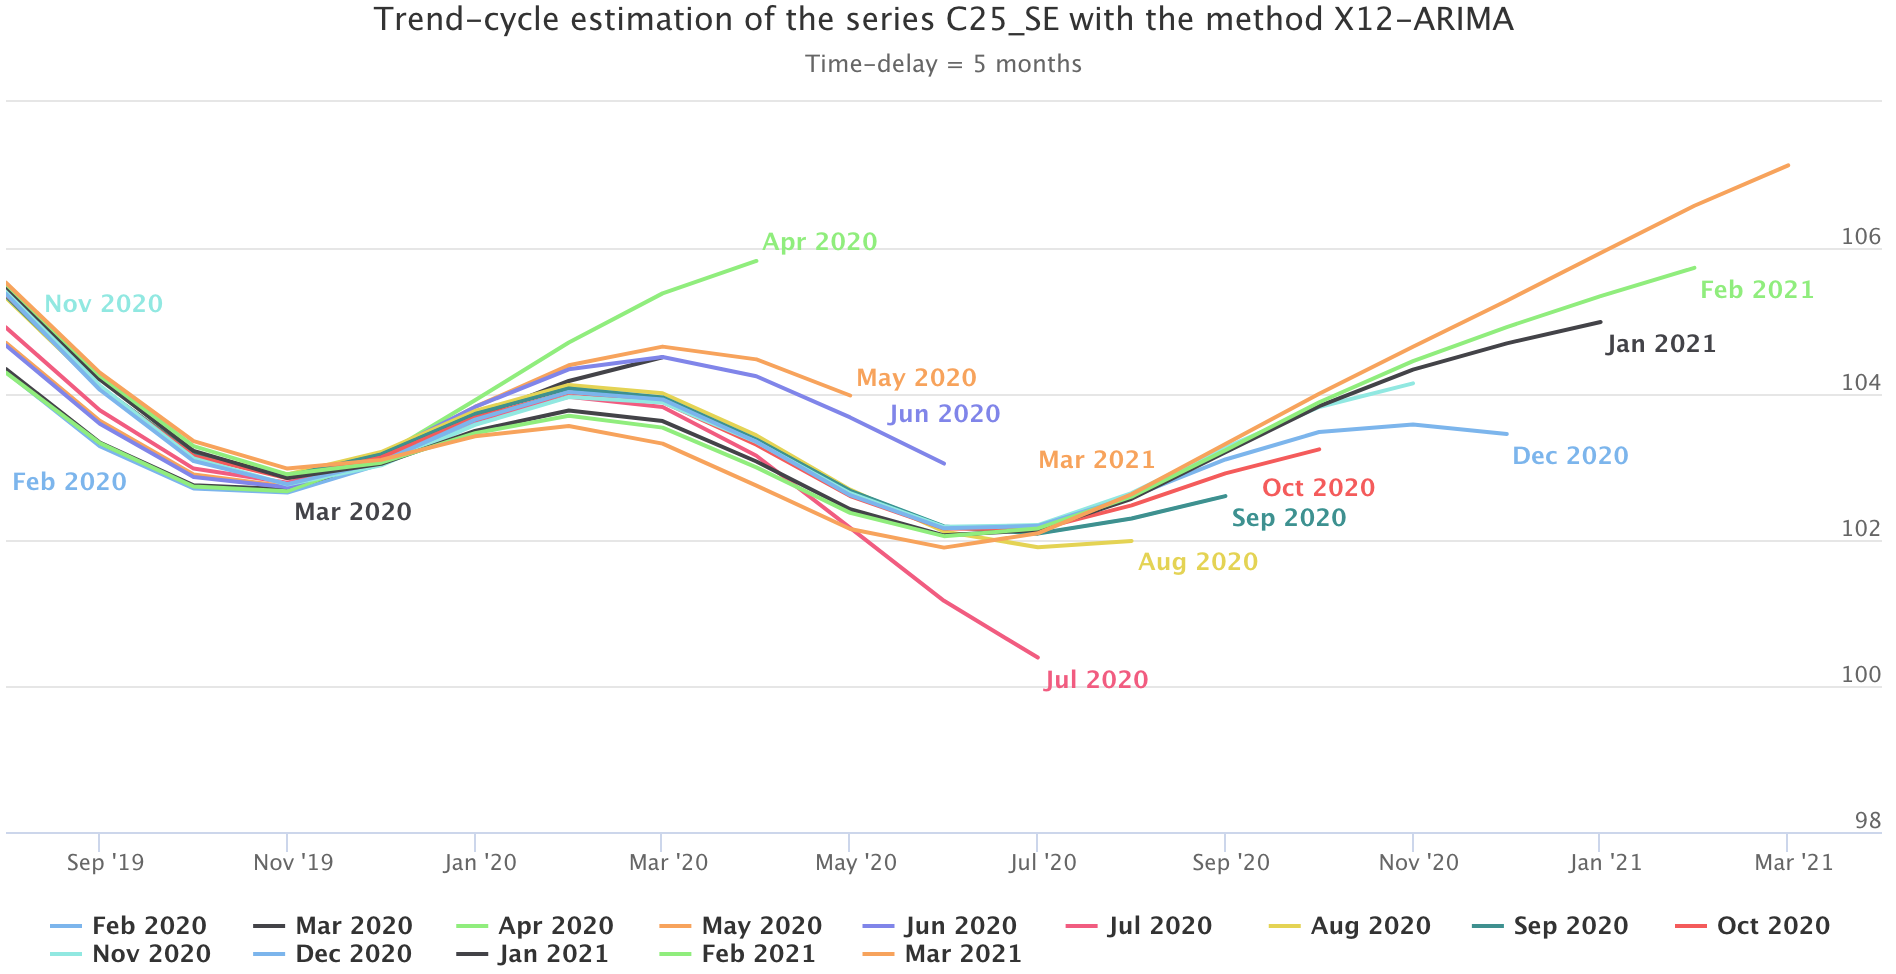
\includegraphics[height = 0.5\paperheight]{img/C25SE_x13}
\end{frame}

\begin{frame}{}
\protect\hypertarget{section}{}
\centering

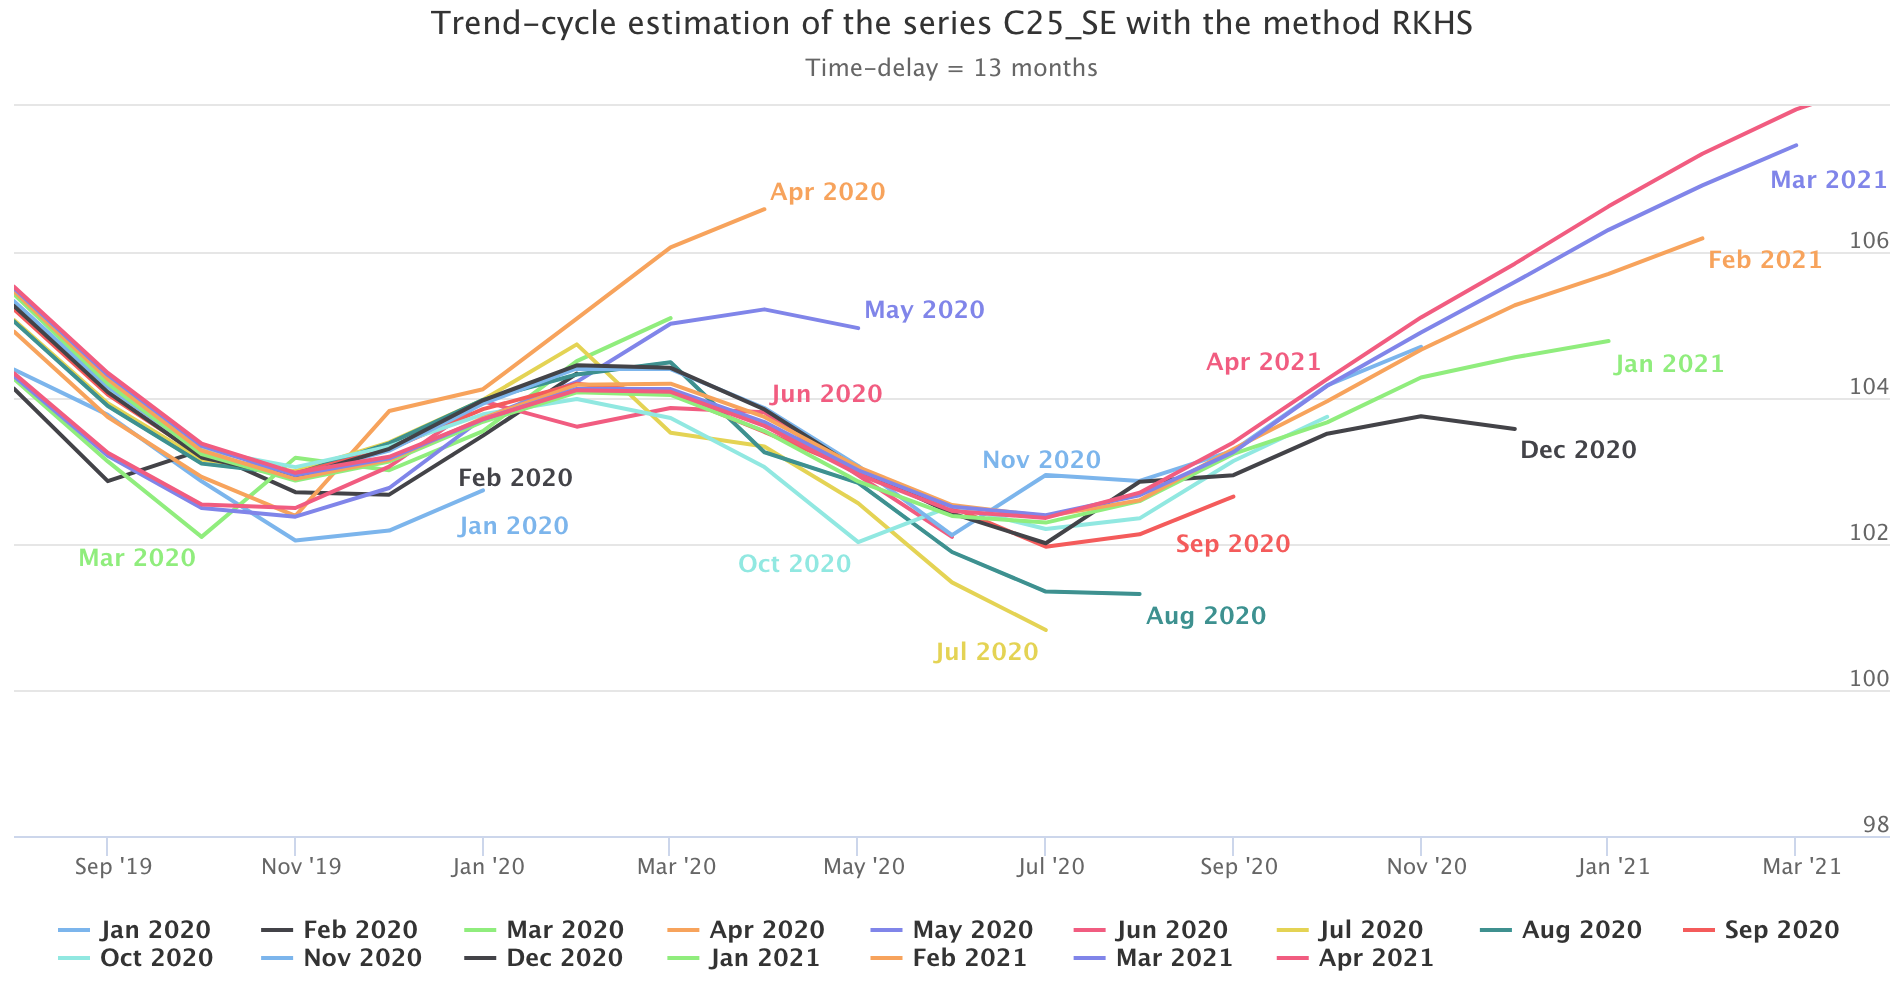
\includegraphics[height = 0.5\paperheight]{img/C25SE_rkhs}
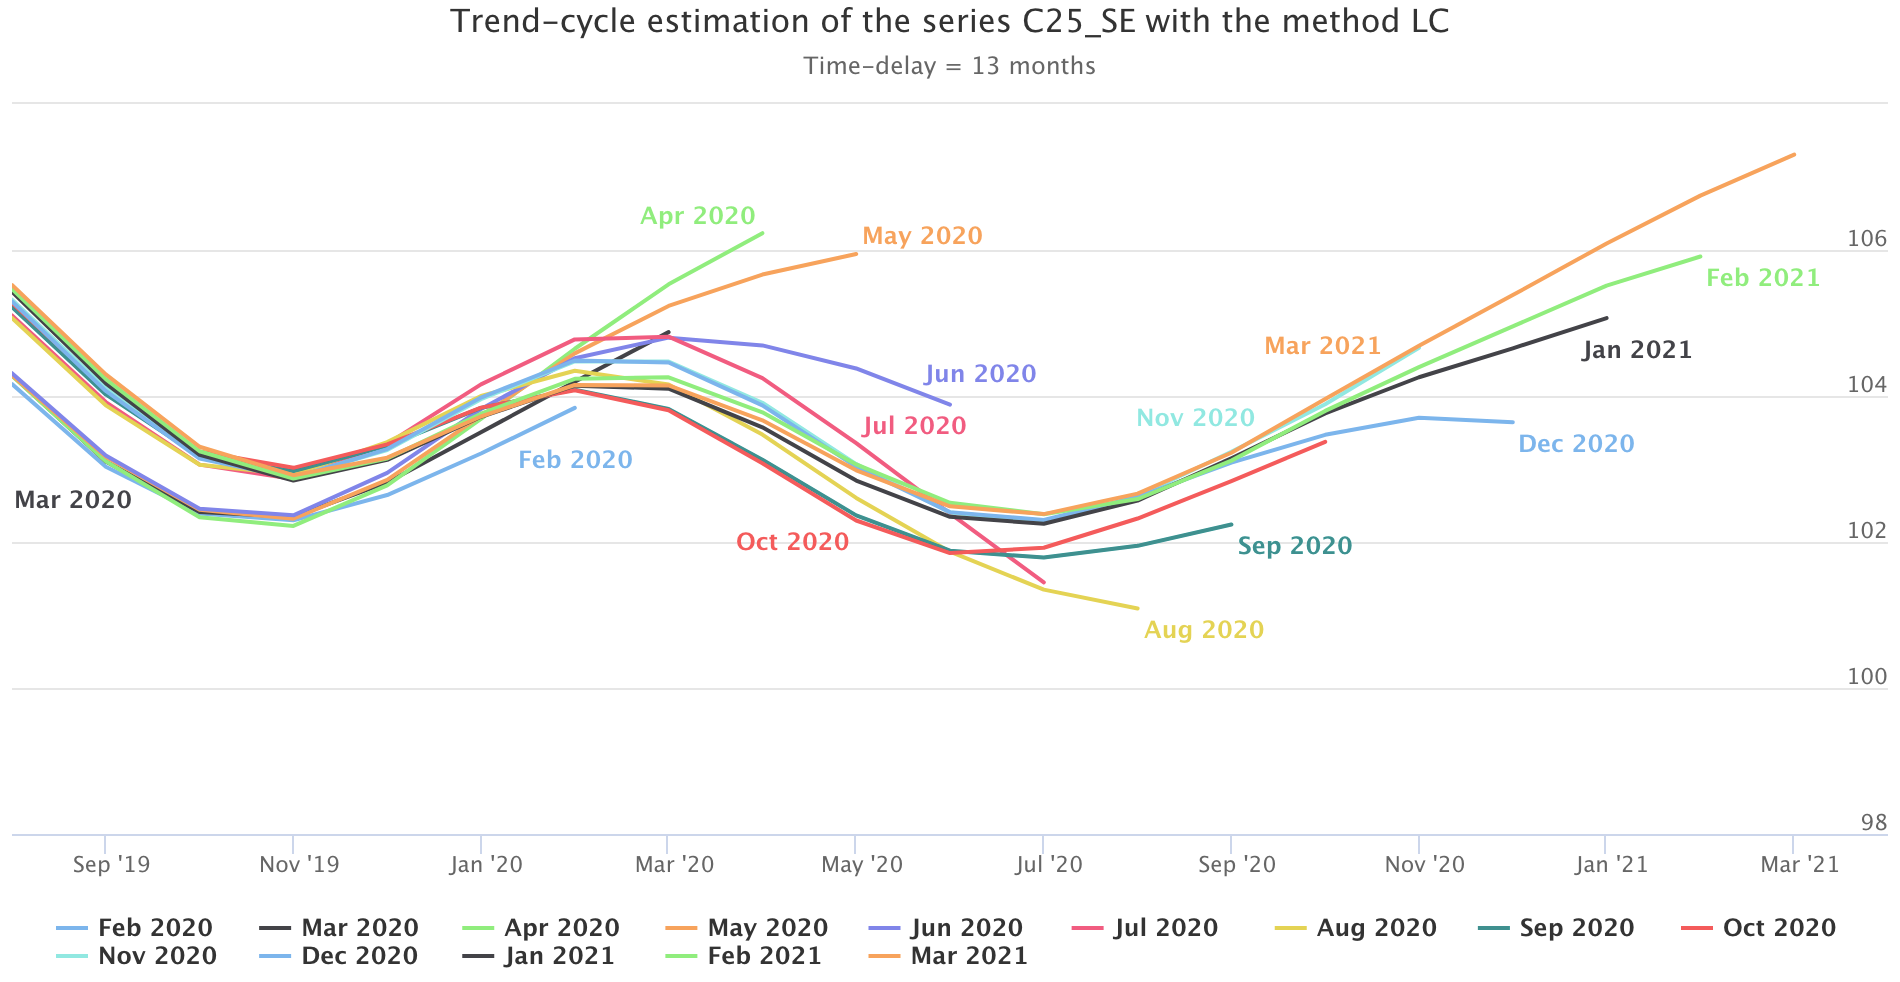
\includegraphics[height = 0.5\paperheight]{img/C25SE_lc}
\end{frame}

\begin{frame}{}
\protect\hypertarget{section-1}{}
\centering

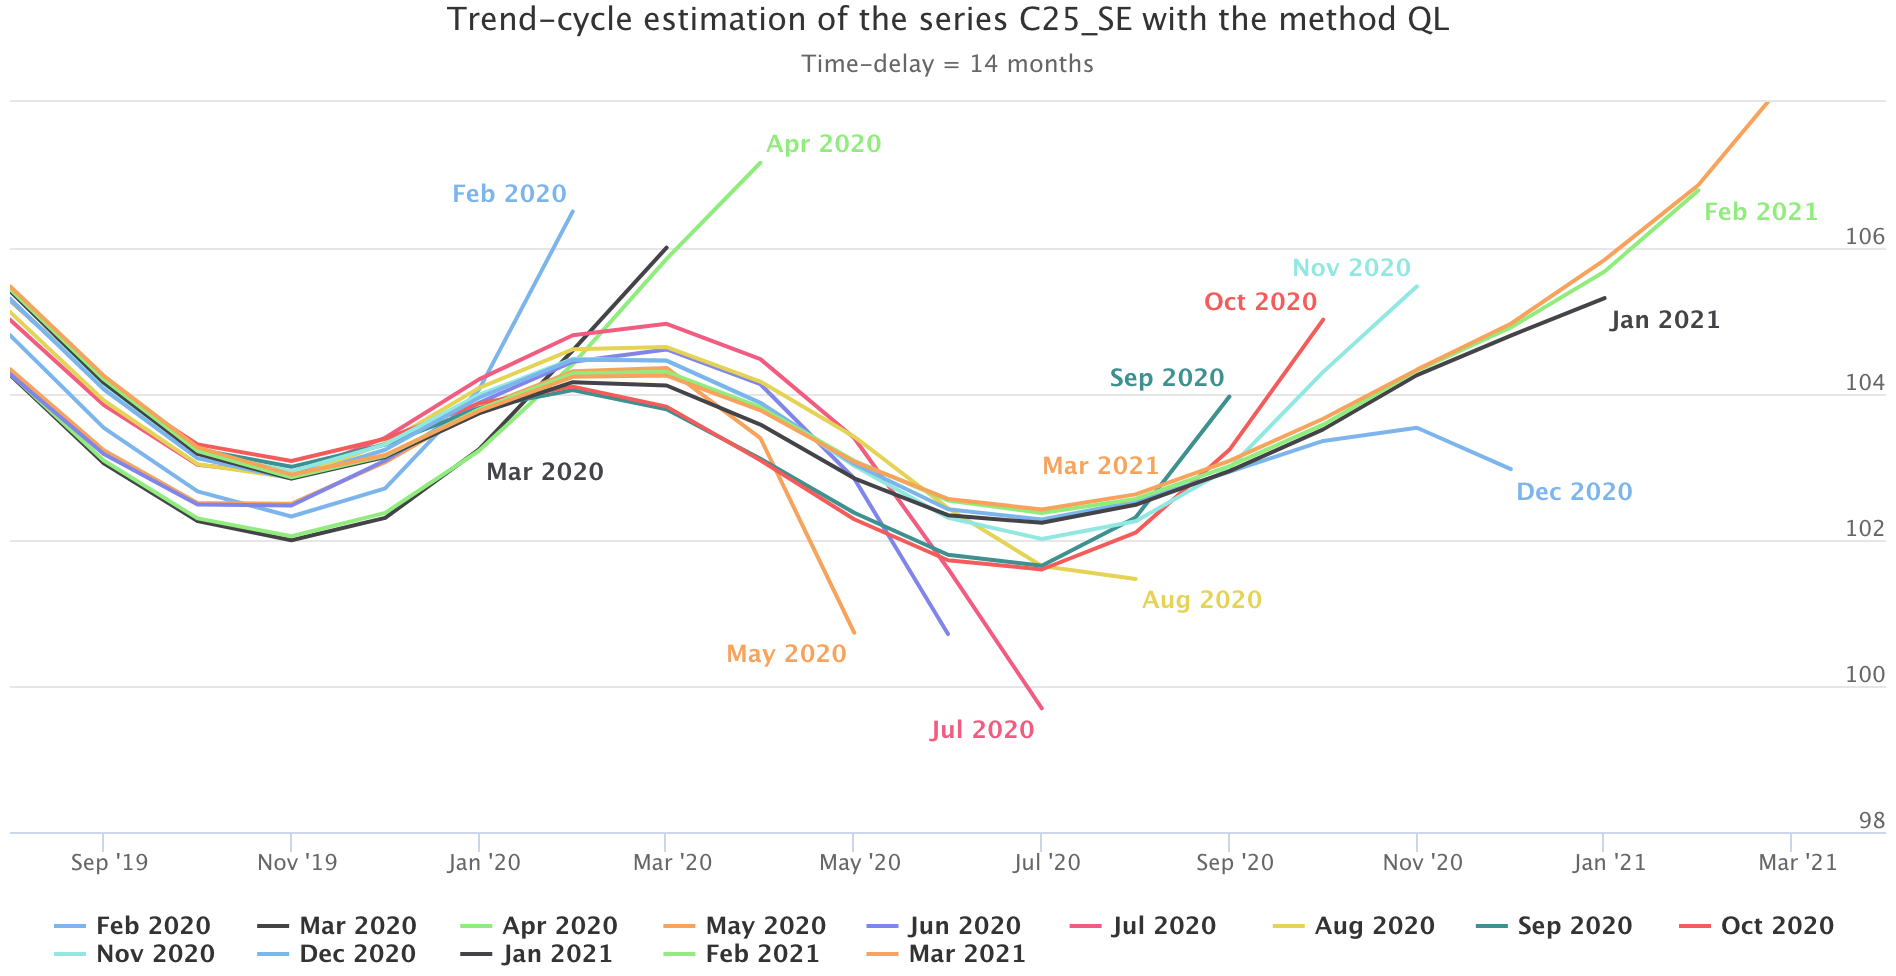
\includegraphics[height = 0.5\paperheight]{img/C25SE_ql}
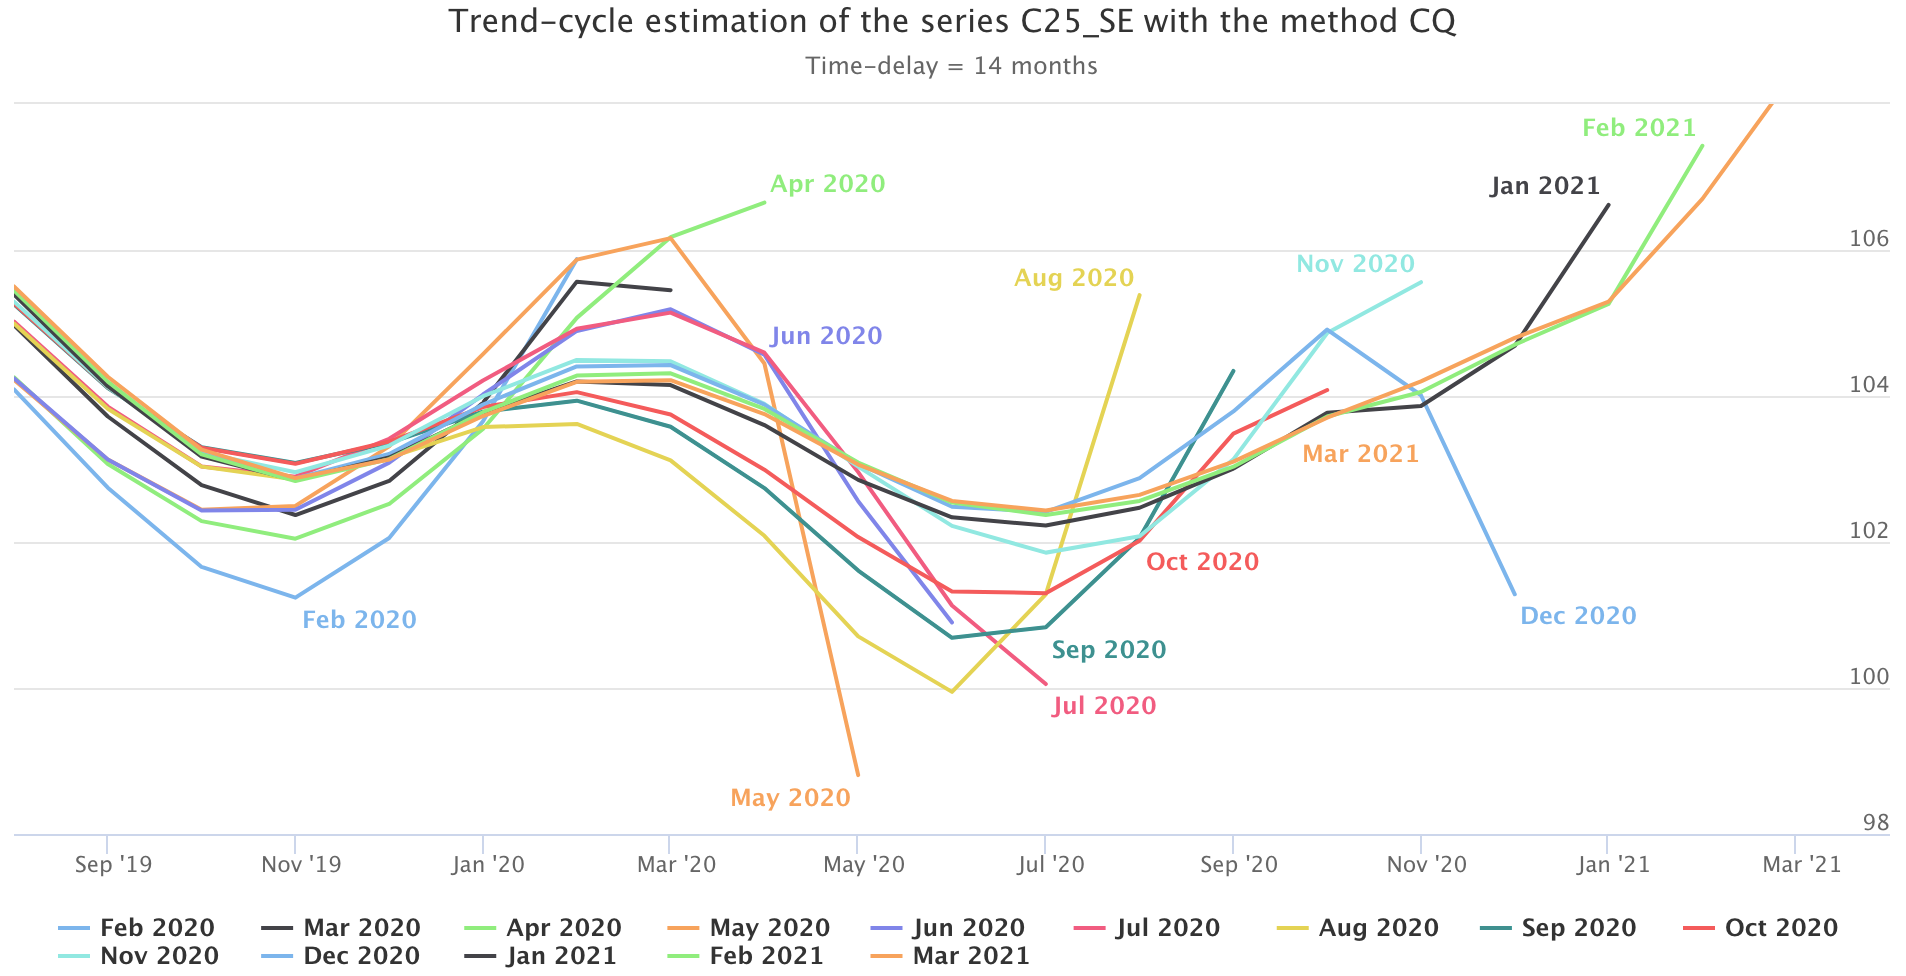
\includegraphics[height = 0.5\paperheight]{img/C25SE_cq}
\end{frame}

\begin{frame}{}
\protect\hypertarget{section-2}{}
\centering

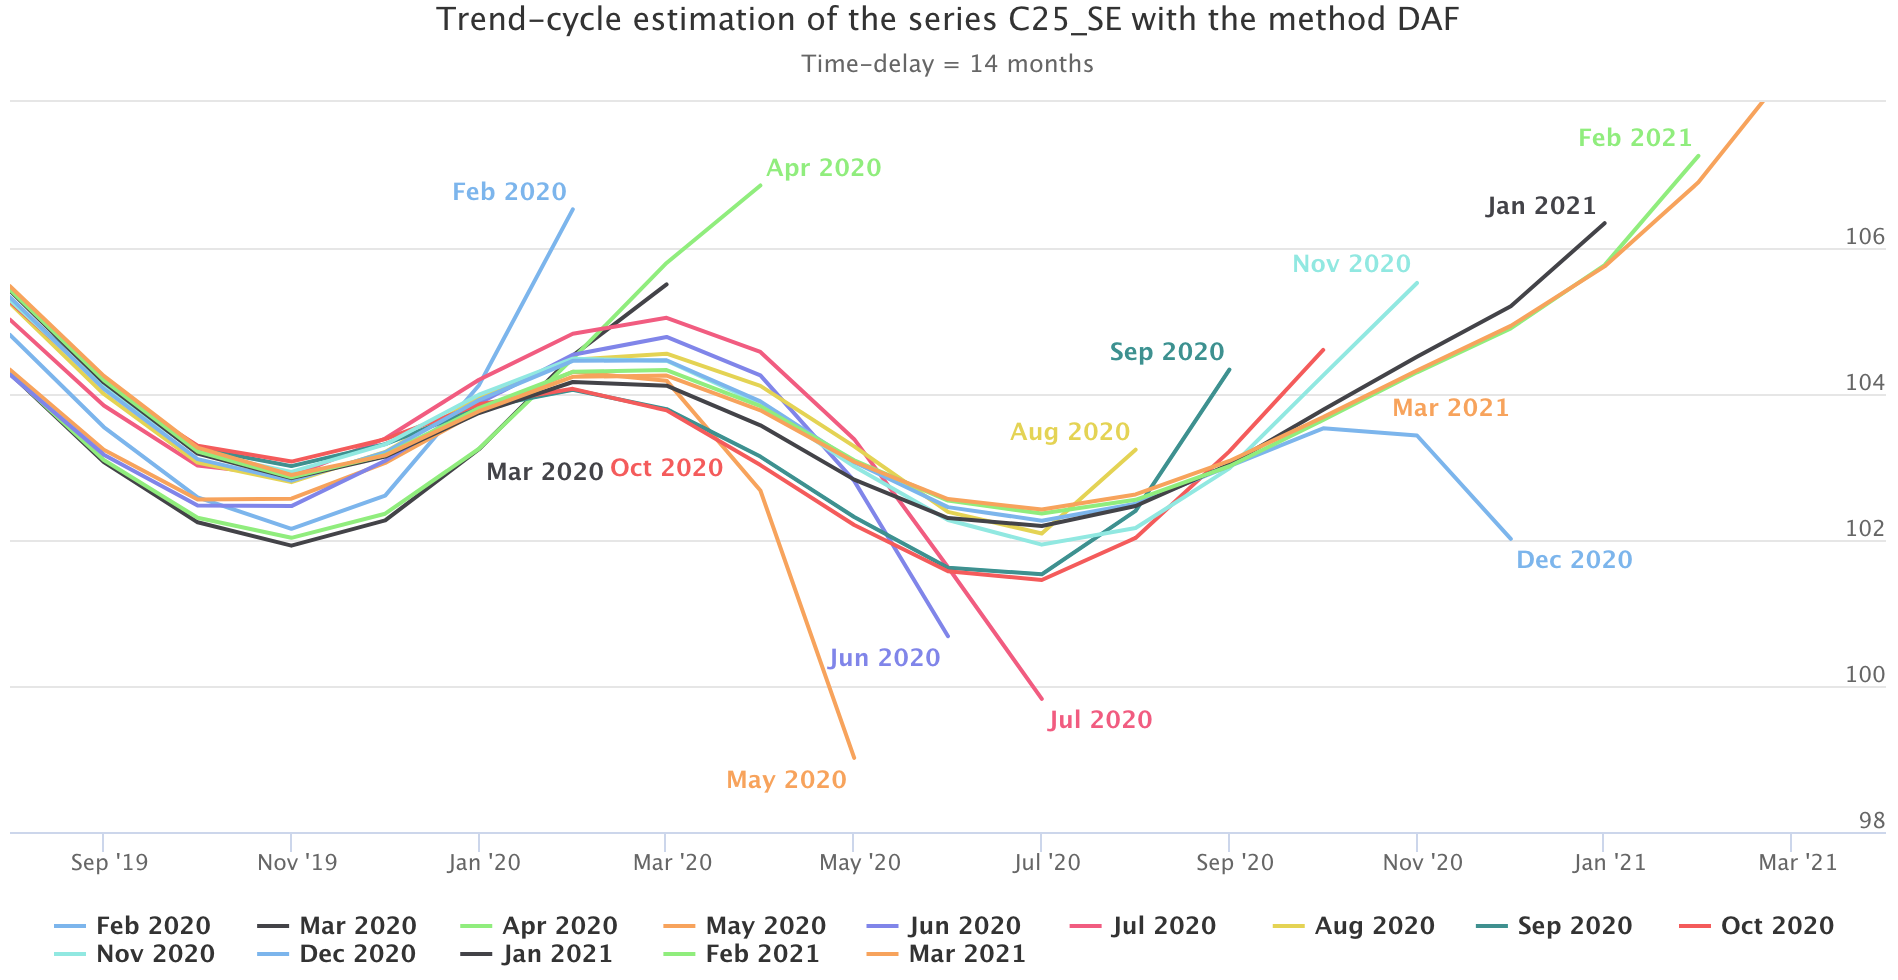
\includegraphics[height = 0.5\paperheight]{img/C25SE_daf}
\end{frame}

\begin{frame}{IPI in the manufacture of cement, lime and plaster (C235)
in Germany (turning point in February 2020)}
\protect\hypertarget{ipi-in-the-manufacture-of-cement-lime-and-plaster-c235-in-germany-turning-point-in-february-2020}{}
\centering

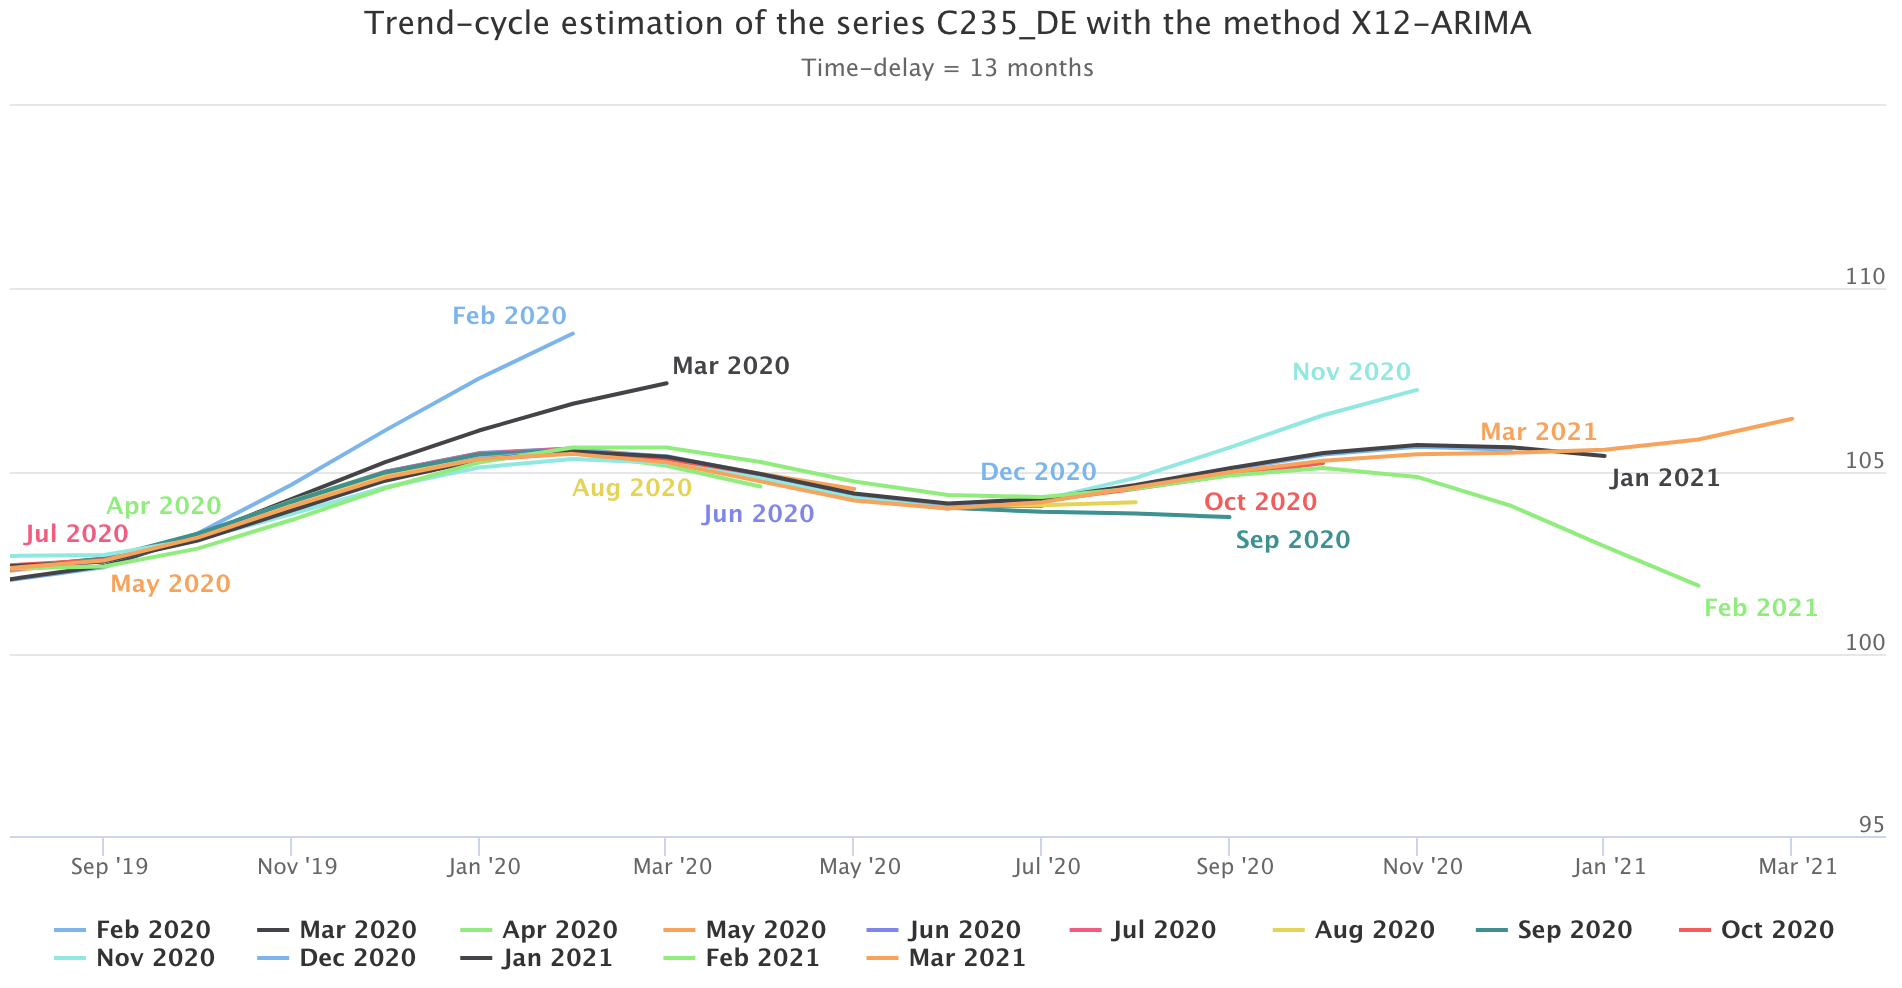
\includegraphics[height = 0.5\paperheight]{img/C235DE_x13}
\end{frame}

\begin{frame}{}
\protect\hypertarget{section-3}{}
\centering

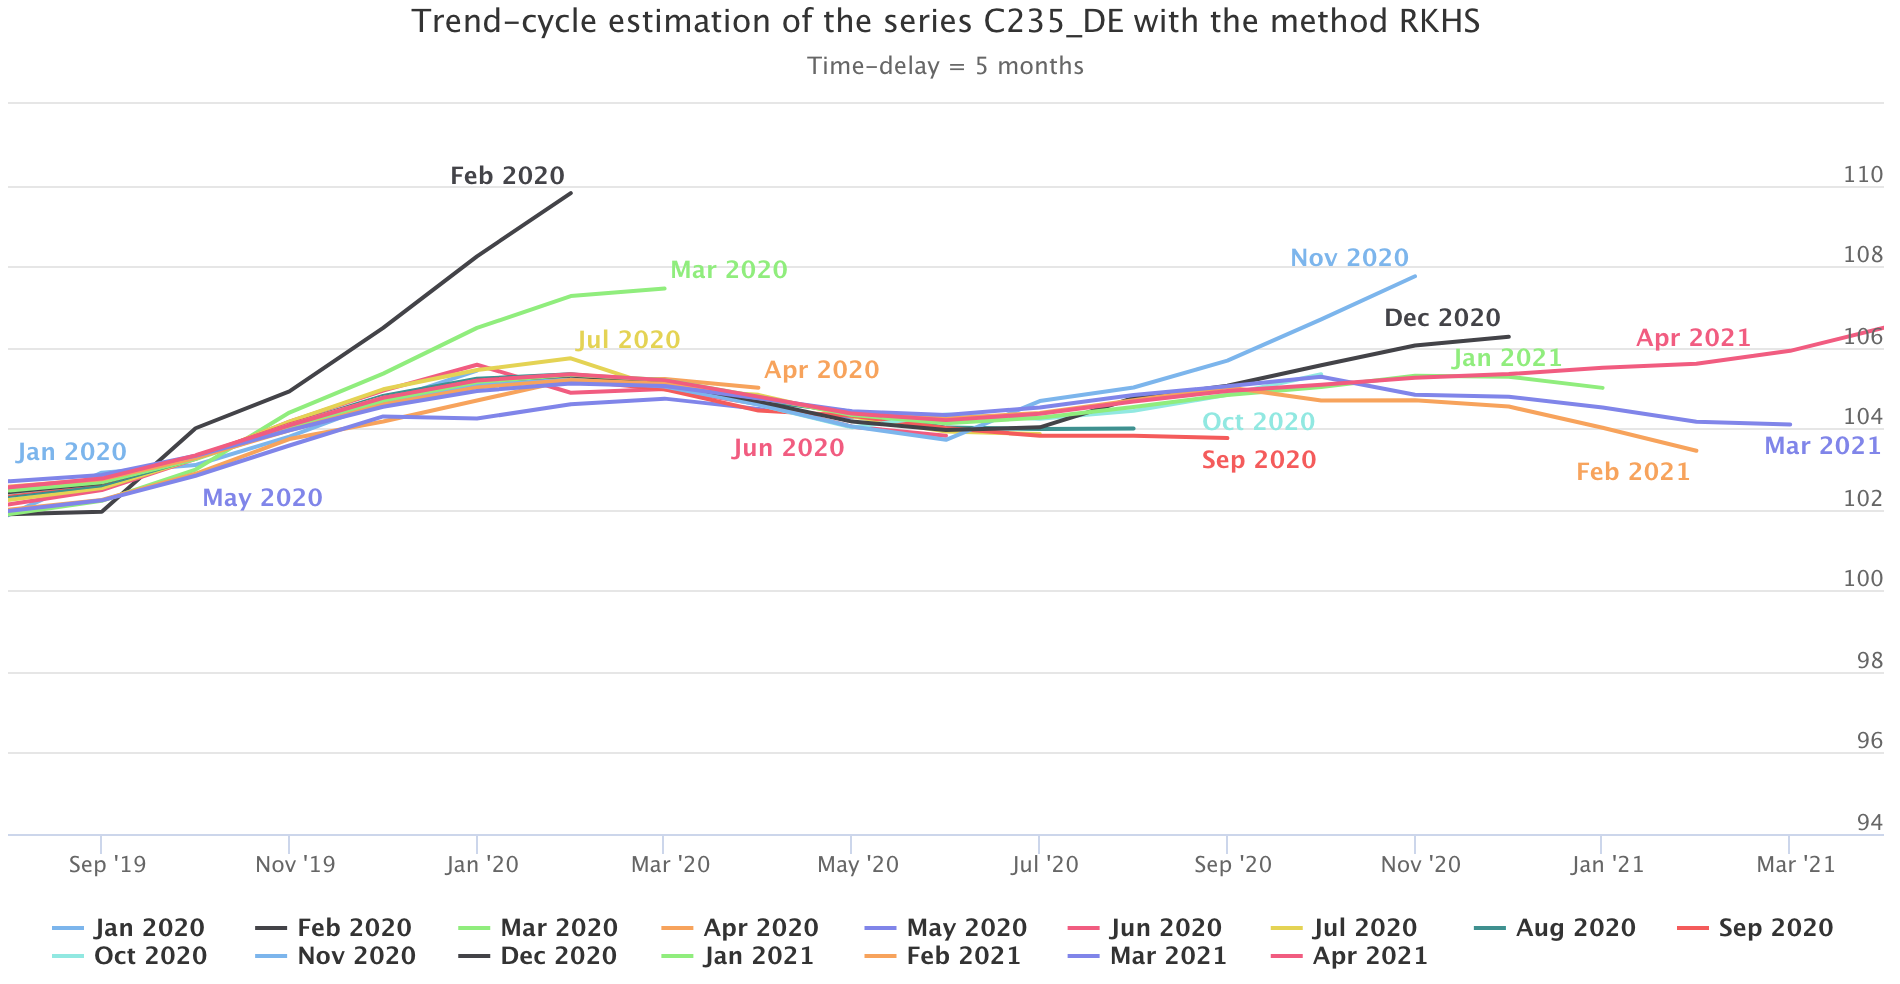
\includegraphics[height = 0.5\paperheight]{img/C235DE_rkhs}
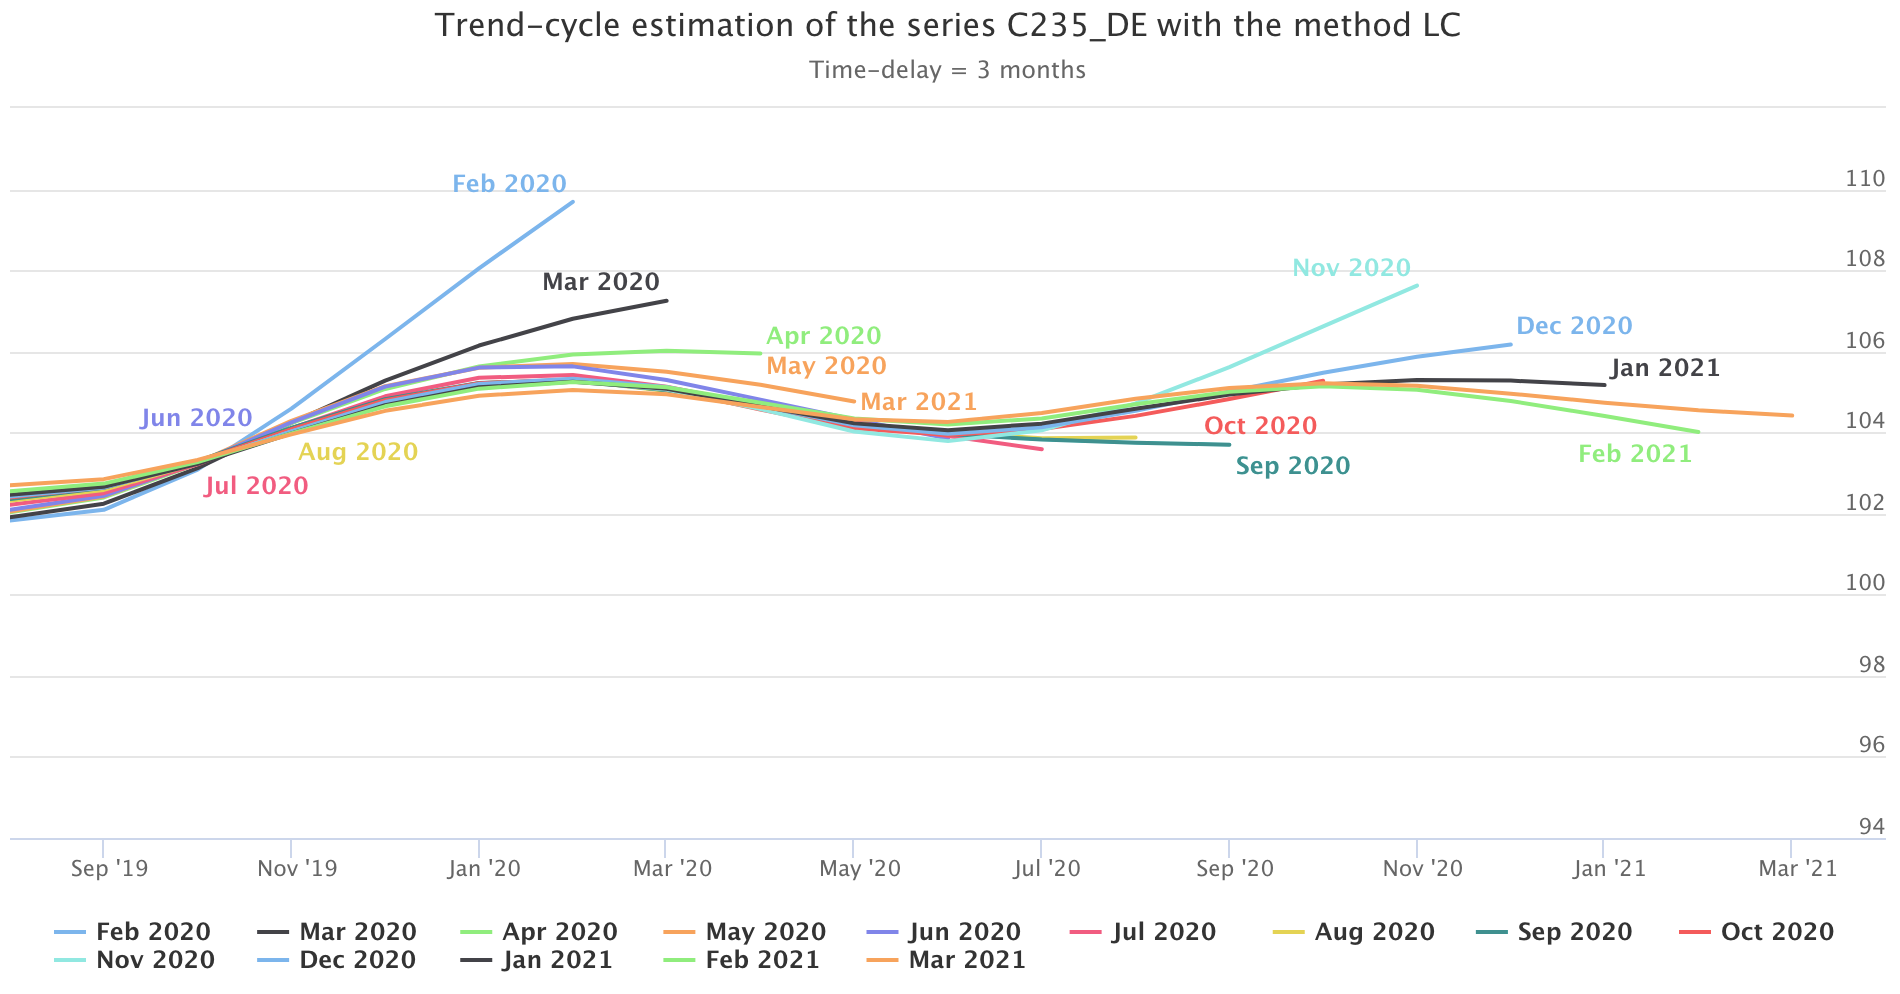
\includegraphics[height = 0.5\paperheight]{img/C235DE_lc}
\end{frame}

\begin{frame}{}
\protect\hypertarget{section-4}{}
\centering

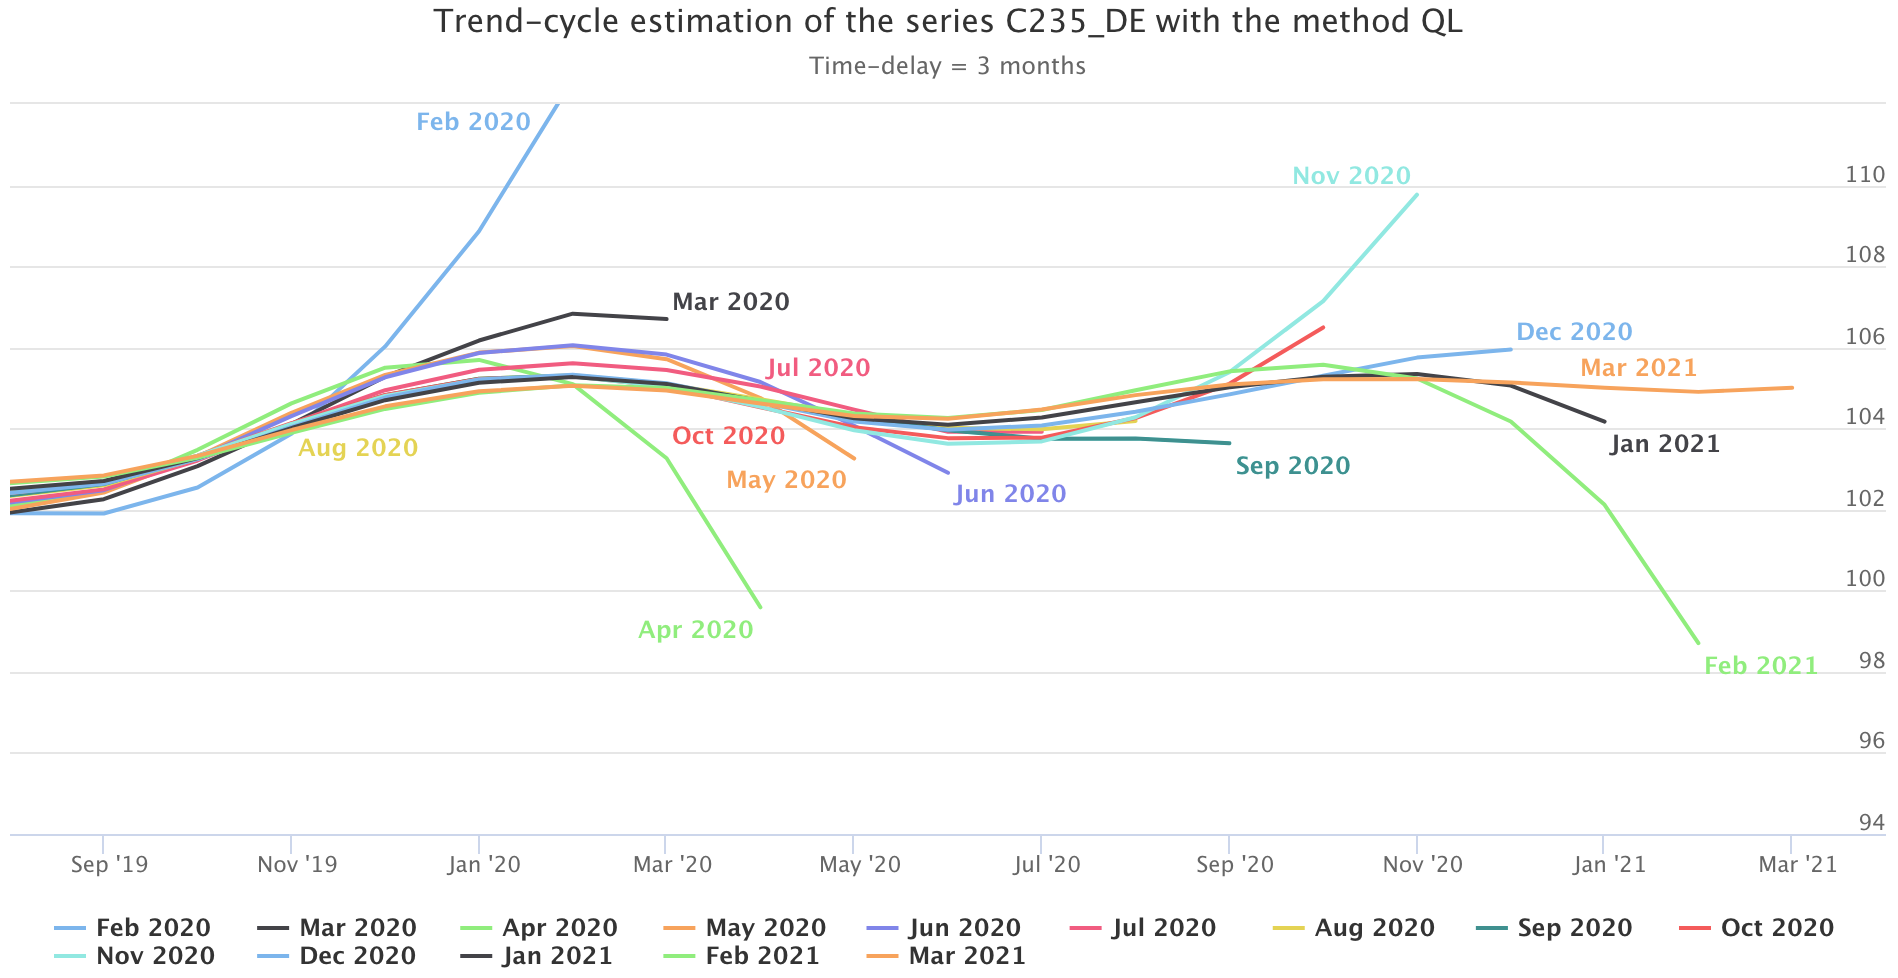
\includegraphics[height = 0.5\paperheight]{img/C235DE_ql}
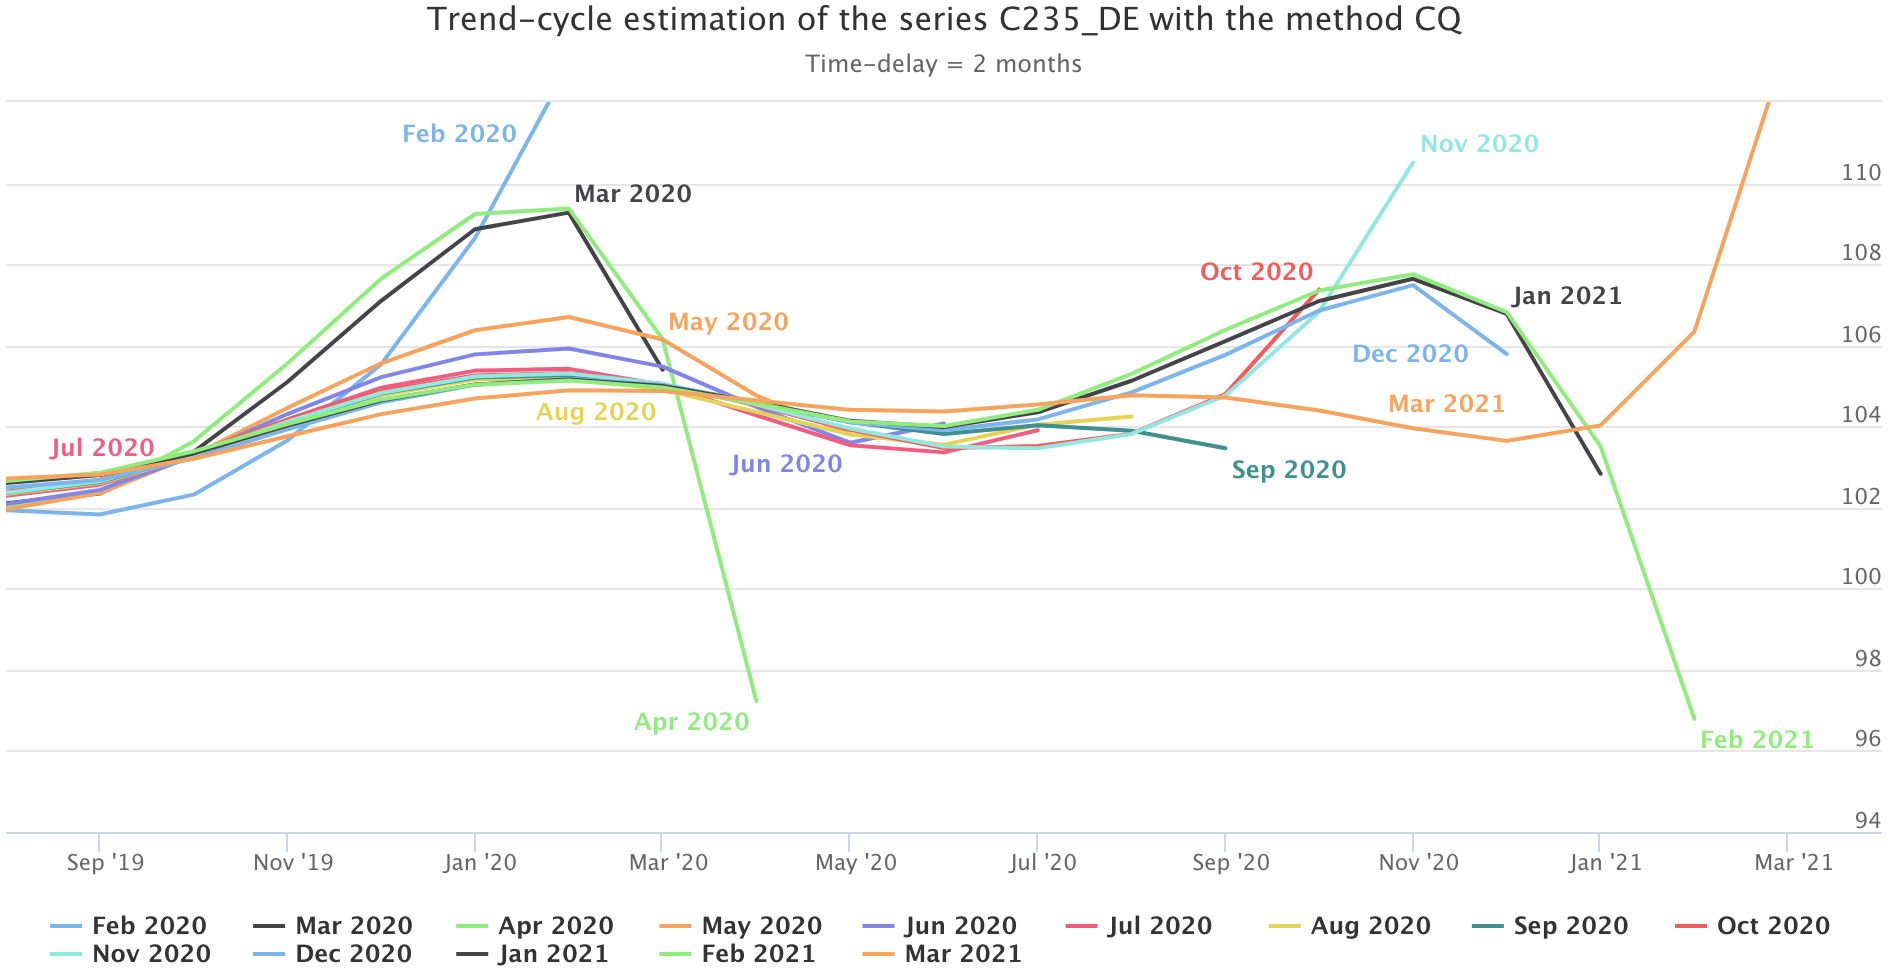
\includegraphics[height = 0.5\paperheight]{img/C235DE_cq}
\end{frame}

\begin{frame}{}
\protect\hypertarget{section-5}{}
\centering

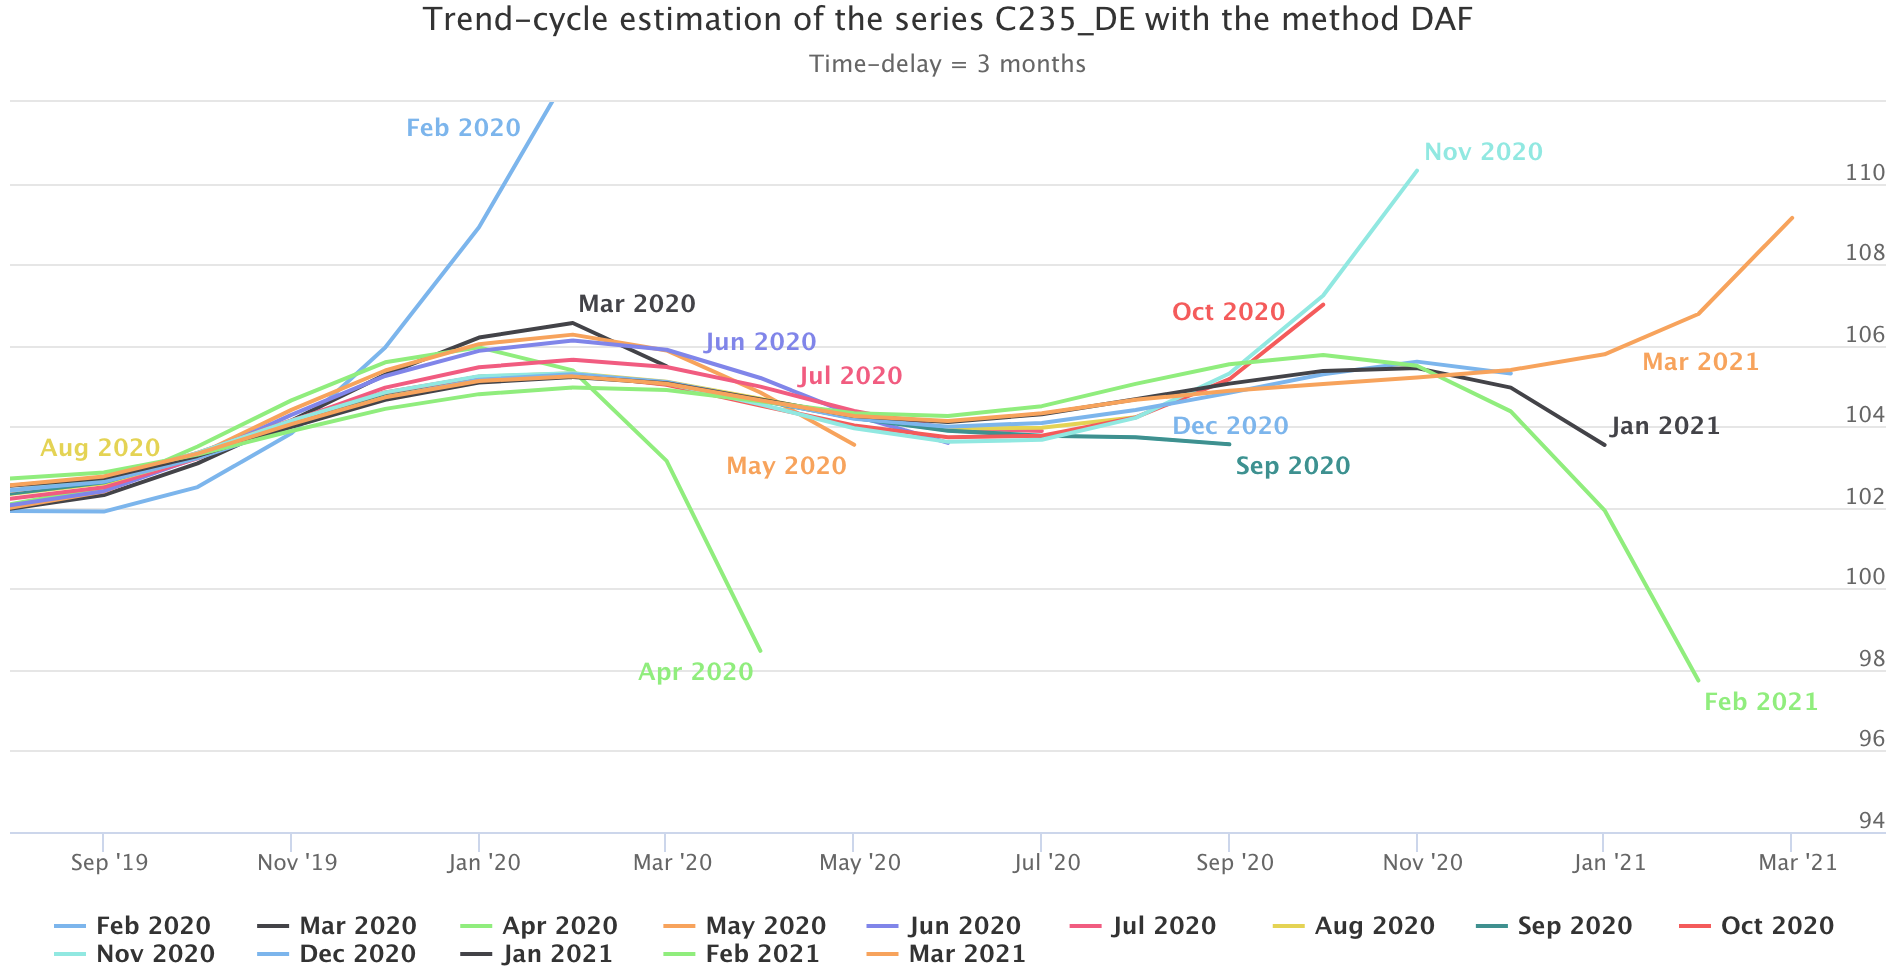
\includegraphics[height = 0.5\paperheight]{img/C235DE_daf}
\end{frame}

\hypertarget{conclusion}{%
\section{Conclusion}\label{conclusion}}

\hypertarget{conclusion-1}{%
\subsection{Conclusion}\label{conclusion-1}}

\begin{frame}[fragile]{Conclusion}
\protect\hypertarget{conclusion-2}{}
\begin{itemize}
\tightlist
\item
  To build asymmetric filters, we can focus on the ones that reproduces
  at most linear trend (excluding QL, CQ and DAF filters)
\end{itemize}

\bigskip \pause

\begin{itemize}
\tightlist
\item
  During the COVID-19, the current X-13-ARIMA algorithm seems to produce
  on average satisfying results
\end{itemize}

\bigskip \pause

\begin{itemize}
\tightlist
\item
  In some cases, we could prefer others trend-cycle filters
  \faIcon{arrow-circle-right} \texttt{rjdfilters} can help
\end{itemize}
\end{frame}

\begin{frame}{What next\bcquestion}
\protect\hypertarget{what-next}{}
\begin{itemize}
\tightlist
\item
  More investigations to understand why and when a method performs
  better
\end{itemize}

\pause

\begin{itemize}
\tightlist
\item
  Study on other datasets
\end{itemize}

\pause

Other methods:

\begin{itemize}
\item
  FST can lead to filters that performs better in terms of Fidelity,
  Smoothness, Timeliness than:

  \begin{itemize}
  \item
    RKHS filters with same polynomial constraints
  \item
    LC filters with same polynomial constraints
  \end{itemize}

  \faIcon{arrow-circle-right} Study of those moving averages?
\end{itemize}

\pause

\begin{itemize}
\tightlist
\item
  Direct Filter Approach (Wildi and McElroy (2019)), Cascade Linear
  Filter (Dagum and Luati (2008)), etc.
\end{itemize}

\pause

\begin{itemize}
\tightlist
\item
  Impact of outliers? Study of robust methods?
\end{itemize}
\end{frame}

\begin{frame}{Thanks for your attention}
\protect\hypertarget{thanks-for-your-attention}{}
\begin{columns}
\begin{column}{0.6\textwidth} 
\faIcon{r-project} package: \href{https://github.com/palatej/rjdfilters}{\faGithub{} palatej/rjdfilters}
\end{column}
\begin{column}{0.4\textwidth}
About me: \href{https://github.com/AQLT}{\faGithub{} AQLT}  
\end{column}
\end{columns}

\textbf{Bibliography}: \footnotesize

\hypertarget{refs}{}
\begin{CSLReferences}{1}{0}
\leavevmode\hypertarget{ref-dagumbianconcini2008}{}%
Dagum, Estela Bee, and Silvia Bianconcini. 2008. {``{The Henderson
Smoother in Reproducing Kernel Hilbert Space}.''} \emph{Journal of
Business \& Economic Statistics} 26: 536--45.
\url{https://ideas.repec.org/a/bes/jnlbes/v26y2008p536-545.html}.

\leavevmode\hypertarget{ref-cascadeFilter}{}%
Dagum, Estela Bee, and Alessandra Luati. 2008. {``A Cascade Linear
Filter to Reduce Revisions and False Turning Points for Real Time
Trend-Cycle Estimation.''} \emph{Econometric Reviews} 28 (1-3): 40--59.
\url{https://doi.org/10.1080/07474930802387837}.

\leavevmode\hypertarget{ref-ch15HBSA}{}%
Grun-Rehomme, Michel, Fabien Guggemos, and Dominique Ladiray. 2018.
{``Asymmetric Moving Averages Minimizing Phase Shift.''} \emph{Handbook
on Seasonal Adjustment}.
\href{https://ec.europa.eu/eurostat/web/products-manuals-and-guidelines/-/KS-GQ-18-001}{ec.europa.eu/eurostat/web/products-manuals-and-guidelines/-/KS-GQ-18-001}.

\leavevmode\hypertarget{ref-proietti2008}{}%
Proietti, Tommaso, and Alessandra Luati. 2008. {``Real Time Estimation
in Local Polynomial Regression, with Application to Trend-Cycle
Analysis.''} \emph{Ann. Appl. Stat.} 2 (4): 1523--53.

\leavevmode\hypertarget{ref-trilemmaWMR2019}{}%
Wildi, Marc, and Tucker McElroy. 2019. {``The Trilemma Between Accuracy,
Timeliness and Smoothness in Real-Time Signal Extraction.''}
\emph{International Journal of Forecasting} 35 (3): 1072--84.
\url{https://EconPapers.repec.org/RePEc:eee:intfor:v:35:y:2019:i:3:p:1072-1084}.

\end{CSLReferences}
\end{frame}

\end{document}
